% vim: set spelllang=fr foldmethod=marker:
\section{Comparaison des trois méthodes de sélection}

    \subsection{Mise en place des simulations}

        \subsubsection{Modèle utilisé}

Le modèle utilisé dans cette section est similaire à celui employé au \chapref{sa} (défini en \ssref{sa:ssec:modelsim}).
Tout comme alors, le logiciel \nsii a été mis en œuvre.
Le cluster est composé d'une grille carrée de cent capteurs, avec le \ch en son centre (soit cent-un capteurs au total; voir \figref{sa:fig:grille}).

La \tabref{sd:table:param} récapitule les principaux paramètres impliqués dans l'exécution des instances.
\begin{table}[ht]
    \centering
    \caption{Paramètres de simulation}\label{sd:table:param}
    \medskip
    \begin{tabular*}{\textwidth}{l@{\hspace{.5em}}c}
        \toprule
        \textsc{Paramètre}                                          & \textsc{Valeur}        \\
        \midrule
        Durée de la simulation                                      & 3\,600~secondes        \\
        Nombre de capteurs                                          & 100 (+~\ch)            \\
        Nombre de \cns                                              & 7--10 (selon scénario) \\
        Nombre de nœuds compromis                                   & 1                      \\
        Fréquence de renouvellement des \cns                        & toutes les 10~secondes \\
        Durée de la période initiale pour la sélection démocratique & 60~secondes            \\
        Mobilité des nœuds                                          & nulle                  \\
    \end{tabular*}
    \begin{tabular*}{\textwidth}{m{.4\textwidth}c@{\hspace{2.5em}}c}
        \midrule
        \multirow{2}{*}{\textsc{Paramètre}} & \textsc{Valeur}                    & \textsc{Valeur}           \\
                                            & \textsc{(nœuds normaux)}           & \textsc{(nœud compromis)} \\
        \midrule
        Taux d'émission                     & 1~ko/s                             & 35~ko/s                   \\
        Taille des paquets                  & 500~octets                         & 100~octets                \\
        Intervalle                          & aléatoire (\textsc{Poisson})       & constant                  \\
        Cons. énergétique en émission       & 0,660~W                            & 0,660~W                   \\
        Cons. énergétique en réception      & 0,395~W                            & non pris en compte        \\
        Quantité initiale d'énergie         & 10~\joule\ --- $\infty$ (sel. sc.) & $\infty$                  \\
        \bottomrule
    \end{tabular*}
\end{table}

Un «scénario» se caractérise par le choix d'un processus de renouvellement des \cns, par le nombre de \cns sélectionnés à chaque tour, et par le montant d'énergie initialement attribué aux capteurs.
Sauf indication contraire, tous les résultats numériques présentés dans cette section sont des moyennes calculées à partir des valeurs de dix instances distinctes (pour chaque scénario).
Ces instances sont différenciées par les valeurs utilisées pour initialiser le générateur de nombres pseudo-aléatoires de \nsii, et (le cas échéant) celui utilisé par les nœuds pour la sélection des \cns.

Les moyennes sur les capteurs sont calculées à partir des valeurs des quatre-vingt-dix-neuf nœuds «sains».
Le \ch ainsi que le nœud compromis sont dotés d'une réserve d'énergie illimitée pour les simulations:
\begin{itemize}
    \item le \ch parce qu'il est indispensable au fonctionnement du cluster, et que sur une instance réelle, l'épuisement de sa batterie se traduirait par la désignation immédiate d'un remplaçant; de plus, il reçoit les paquets «utiles» de tous les nœuds, et sa consommation en énergie, très importante, viendrait «fausser» les moyennes que nous cherchons à étudier ici;
    \item le nœud compromis parce que nous ne souhaitons pas qu'il arrête d'émettre au cours du déroulement de notre scénario; et parce que les nombreux paquets qu'il émet lui font là aussi dépenser une énergie qui viendrait fausser les moyennes observées. Outre le contexte des simulations, il est à noter qu'un tel cas est plausible, par exemple, si l'attaquant substitue au nœud ciblé un appareil plus puissant (un ordinateur portable par exemple) sur une longue durée: le nœud compromis peut alors se retrouver affranchi des contraintes en énergie auxquelles sont soumis les autres capteurs.
\end{itemize}

        \subsubsection{Choix du simulateur}

Le simulateur utilisé au \chapref{sa} est \nsii~\cite{ns2}; celui employé au \chapref{se} est \nsiii~\cite{ns3}.
\nsiii est une version plus récente de \nsii.
Basé sur les mêmes mécanismes, le logiciel a été complètement réécrit, et les langages utilisés pour définir les scénarios de simulation ne sont plus les mêmes (Tcl pour \nsii, \cpp (éventuellement Python) pour \nsiii).
Ce changement radical a pour conséquence l'absence de compatibilité descendante avec \nsii.

Il semble nécessaire d'expliquer ici en quelques mots le choix des logiciels utilisés.
Nous avons commencé à travailler sur \nsii, sans vraiment étudier d'alternative dans un premier temps.
Cependant les travaux de simulation présentés aux chapitres~\ref{chap:sa} et~\ref{chap:se} n'ont pas été réalisé d'une seule traite, mais avec plusieurs mois d'écart.
Durant cette période, nous avons pensé abandonner \nsii pour nous tourner vers \nsiii, plus récent, mieux conçu, mieux documenté (bien que moins complet à ce jour, mais cela ne nous a pas porté préjudice pour les simulations réalisées).

Malheureusement, nous nous sommes heurtés à des problèmes de performances: une instance d'une durée (virtuelle) d'une demi-heure, sous \nsiii, nous a pris une semaine entière à exécuter, sur un ordinateur récent.
Malgré nos requêtes sur la liste ainsi que sur le canal de discussion associés au simulateur, nous n'avons pas réussi à contourner cet écueil.
Nous ne savons toujours pas, à la publication de cet ouvrage, si le problème vient d'une erreur introduite avec notre code, ou bien s'il s'avère simplement que \nsiii se prête mal à ce type de scénarios.
Certaines sources semblent affirmer qu'avec \nsiii, «le passage à l'échelle n'est pas efficace pour les WSN»\,\footnote{«\textit{[\nsiiinxs] does not scale well for WSNs}»~\cite{AAAHN12}}, ce qui tendrait à conforter la seconde hypothèse.

Devant la durée très (trop) importante de l'exécution des simulations désirées, nous sommes revenus vers \nsii pour comparer dans ce chapitre l'ensemble des processus de sélection proposés.

    \subsection{Résultats numériques}


        \subsubsection{Consommation énergétique}
\begin{figure}[H]
    \centering
    \includegraphics{\chapterfig/plot_sd_consumptionXtime.pdf}
    \caption{Moyenne de l'énergie consommée par les capteurs au cours du temps (énergie initiale: $\infty$)}\label{sd:fig:cons-inf}
\end{figure}
\begin{figure}[H]
    \centering
    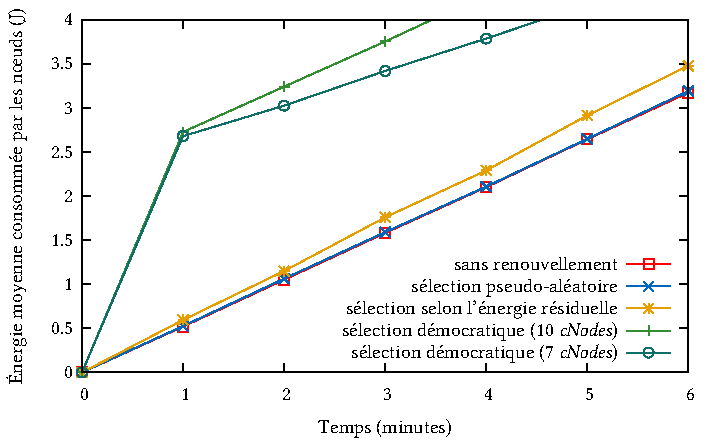
\includegraphics{\chapterfig/plot_sd_consumptionXtime_zoom10.pdf}
    \caption{Moyenne de l'énergie consommée par les capteurs au cours du temps: agrandissement de la vue près de l'origine du repère (énergie initiale: $\infty$)}\label{sd:fig:cons-inf-zoom}
\end{figure}
\begin{figure}[H]
    \centering
    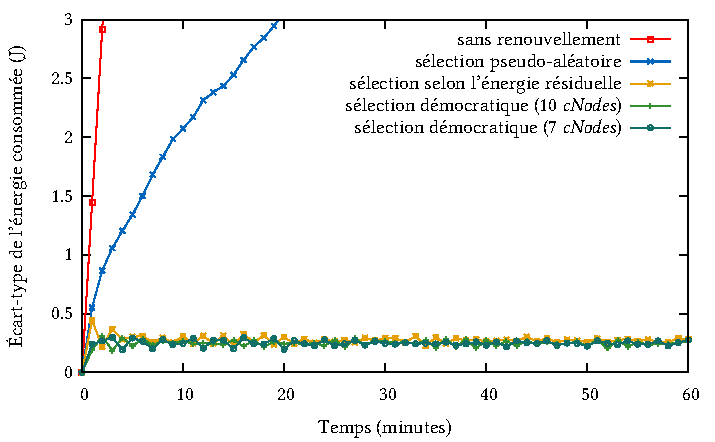
\includegraphics{\chapterfig/plot_sd_stddevXtime.pdf}
    \caption{Écart-type moyen pour l'énergie consommée par les capteurs au cours du temps (énergie initiale: $\infty$)}\label{sd:fig:stddev-inf}
\end{figure}

        \subsubsection{Taux de détection}
\begin{figure}[H]
    \centering
    \includegraphics{\chapterfig/plot_sd_detectionXtime-single_10J.pdf}
    \caption{Taux de détection, pour chaque processus de sélection, au cours du temps (énergie initiale: 10~\joule; valeurs sur une seule instance)}\label{sd:fig:detec-one-10J}
\end{figure}

%CALCUL : probabilité que n cNodes parmi les 10 soient piochés parmi les NON voisins du nœud 12 compromis (code JavaScript)
%function f(n) {
  %if (n<=1)
    %return 1;
  %else
    %return f(n-1)*n;
%}

%function p(k) {
  %m=61;
  %N=100;
  %n=10;
  %Nm=N-m;
  %nk=n-k;

  %ckm = f(m)/(f(k)*f(m-k));
  %cnkNm = f(Nm)/(f(nk)*f(Nm-nk));
  %cnN = f(N)/(f(n)*f(N-n));

  %return ckm*cnkNm/cnN;
%}

%var sum=0;
%for (var i=0;i<=10;i++) {
  %sum+=p(i);
  %console.log(i, p(i)*100);
%}

%Résultats (%) :
%0 0.0036726402702378143 ~ 1/27228
%1 0.07467701882816889
%2 0.6504127446324387
%3 3.19786266110949
%4 9.835850306139795
%5 19.78741649823418
%6 26.383221997645574
%7 23.032971585246138
%8 12.605883097330656
%9 3.907086574026461
%10 0.5209448765368615
La répartition des \cns, lors du processus de sélection aléatoire, suit une loi de probabilité hypergéométrique.
Il est possible de calculer la probabilité pour que $k$ \cns sur les $n=10$ soient choisis parmi les $m=61$ voisins directs du nœud compromis, sur un total de $N=100$ candidats, à l'aide de la formule suivante:
$$P(k) = \frac{{m\choose k}{N-m\choose n-k}}{{N\choose n}}=
\frac{m!}{k!\,(m-k)!}\times\frac{(N-m)!}{(n-k)!\,((N-m)-(n-k))!}\times\frac{n!\,(N-n)!}{N!}$$
La probabilité que le nœud compromis ne soit surveillé par aucun \cn est donc de:
\begin{align*}
    P(0)&=\frac{61!}{0!\,(61-0)!}\times\frac{(100-61)!}{(10-0)!\,((100-61)-(10-0))!}\times\frac{10!\,(100-10)!}{100!}\\
        &\approx3,6\times10^{-5}\approx1/27228
\end{align*}


\begin{figure}[H]
    \centering
    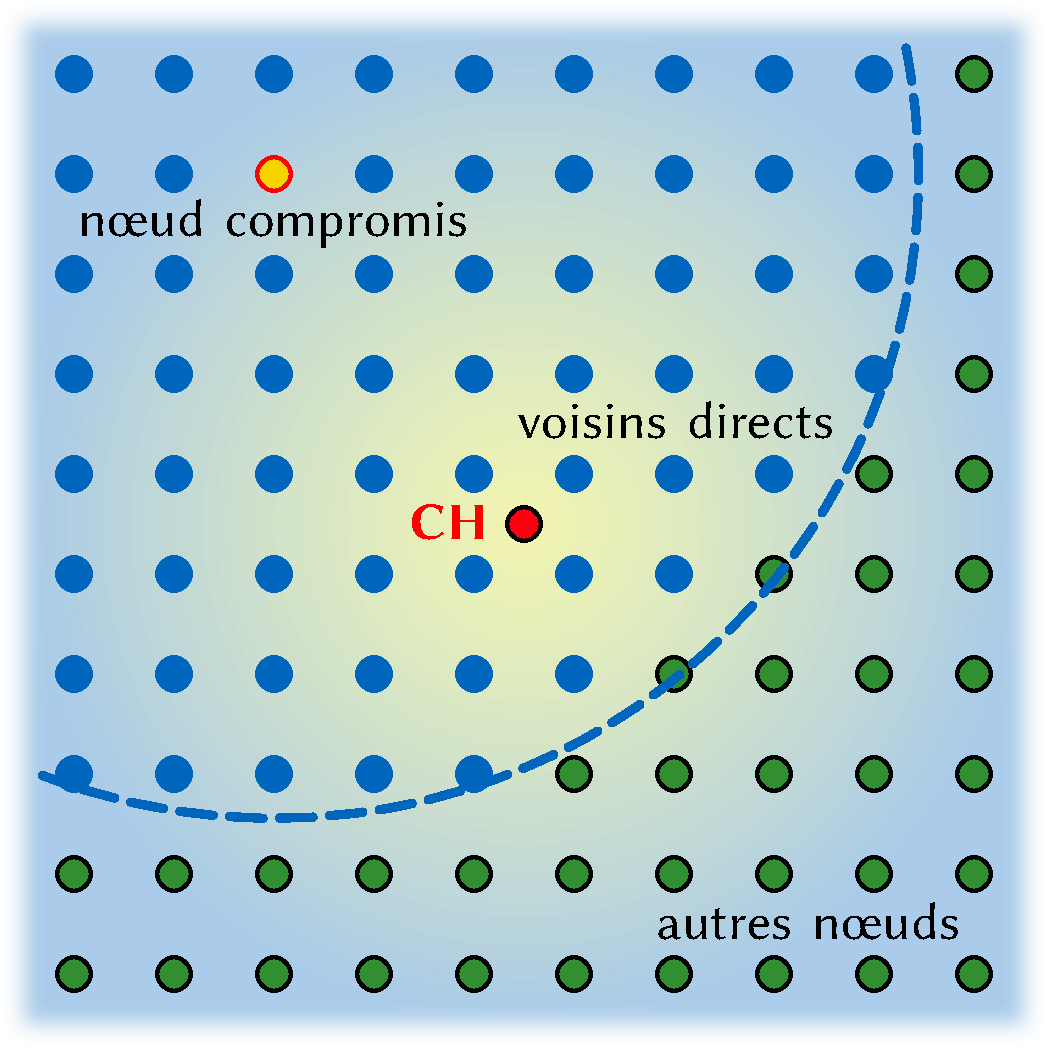
\includegraphics[width=6.5cm]{\chapterfig/WSN_neighbors.pdf}
    \caption{Schéma du cluster représentant la position des soixante-et-un voisins directs (en bleu) du nœud compromis (en jaune) tels que définis dans les simulations réalisées}\label{sd:fig:neighbors}
\end{figure}
\begin{figure}[H]
    \centering
    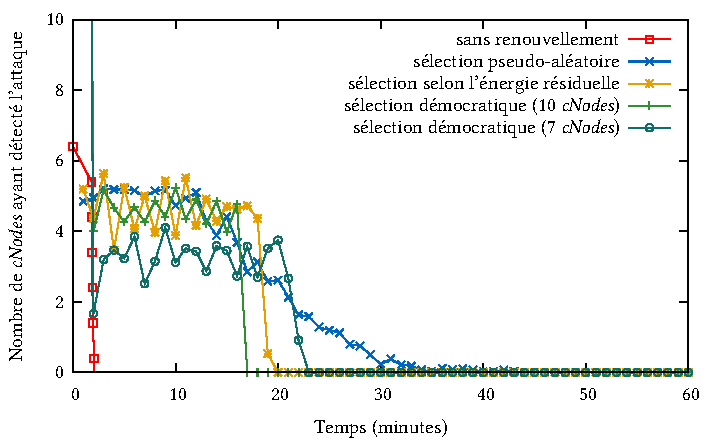
\includegraphics{\chapterfig/plot_sd_detectionXtime-minute_10J.pdf}
    \caption{Taux de détection, pour chaque processus de sélection, au cours du temps (énergie initiale: 10~\joule; valeurs lissées sur une durée d'une minute)}\label{sd:fig:detec-min-10J}
\end{figure}
\begin{figure}[H]
    \centering
    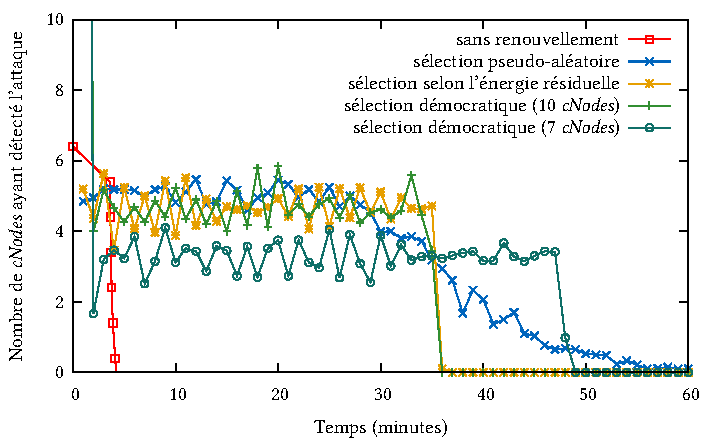
\includegraphics{\chapterfig/plot_sd_detectionXtime-minute_20J.pdf}
    \caption{Taux de détection, pour chaque processus de sélection, au cours du temps (énergie initiale: 20~\joule; valeurs lissées sur une durée d'une minute)}\label{sd:fig:detec-min-20J}
\end{figure}


        \subsubsection{Durée de vie du réseau}
\begin{figure}[H]
    \centering
    \includegraphics{\chapterfig/plot_sd_nbnodesXtime_10J.pdf}
    \caption{Nombre de nœuds en activité au cours du temps pour un montant d'énergie initiale de 10~\joule}\label{sd:fig:nbnodes-10J}
\end{figure}
\begin{figure}[H]
    \centering
    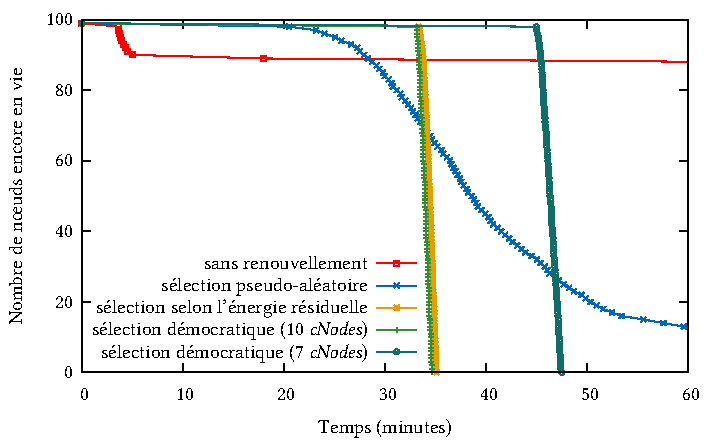
\includegraphics{\chapterfig/plot_sd_nbnodesXtime_20J.pdf}
    \caption{Nombre de nœuds en activité au cours du temps pour un montant d'énergie initiale de 20~\joule}\label{sd:fig:nbnodes-20J}
\end{figure}

    \subsection{Choisir un processus de sélection}
